\documentclass[a4paper,12pt]{article}

\usepackage[T2A]{fontenc}
\usepackage[utf8]{inputenc}
\usepackage[russian]{babel}
\usepackage{amsmath,amssymb}
\usepackage{graphicx}
\usepackage{hyperref}
\usepackage{listings}
\usepackage{caption}
\usepackage{etoolbox}
\usepackage{xcolor}
\usepackage{geometry}
\geometry{margin=2.5cm}

\graphicspath{{../images/}}

\hypersetup{
  colorlinks=true,
  linkcolor=black,
  urlcolor=blue,
  pdftitle={Отчёт по программе доказательства формул IPL}
}

\lstset{
  basicstyle=\ttfamily\small,
  breaklines=true,
  frame=single,
  columns=fullflexible,
  keepspaces=true,
  showstringspaces=false,
  captionpos=b
}

\captionsetup[lstlisting]{%
  skip=0.5em,
  font=small,
  labelfont=bf,
  singlelinecheck=off,
  justification=centering
}
\renewcommand{\lstlistingname}{Листинг}

\newenvironment{listingcenter}{%
  \begin{center}\begin{minipage}{\linewidth}%
}{%
  \end{minipage}\end{center}%
}

\BeforeBeginEnvironment{lstlisting}{\begin{listingcenter}}
\AfterEndEnvironment{lstlisting}{\end{listingcenter}}

\newcommand{\hssnippet}[2]{%
  \begin{listingcenter}%
  \lstinputlisting[style=hs,caption={#2},label={lst:#1}]{snippets/#1}%
  \end{listingcenter}}

\lstdefinestyle{formula}{
  basicstyle=\ttfamily\small,
  breaklines=false,
  frame=single
}

\lstdefinestyle{hs}{
  basicstyle=\ttfamily\small,
  breaklines=true,
  frame=single,
  columns=fullflexible,
  keepspaces=true,
  showstringspaces=false,
  aboveskip=0.5em,
  belowskip=0.5em
}

\begin{document}
\tableofcontents
\newpage

\section{Инструкция пользователя}

Программа \texttt{diploma-exe} проверяет, является ли заданная формула
теоремой интуиционистской пропозициональной логики (IPL). Точка входа ---
функция \texttt{test2} в \texttt{app/Main.hs}:
\hssnippet{main-pipeline.hs}{Точка входа: \texttt{test2} в \texttt{app/Main.hs}}

При положительном ответе строится аннотированное дерево доказательства;
при отрицательном --- контрмодель Kripke.

\subsection{Формат входных данных}

Вход --- текстовый файл с одной формулой IPL. Синтаксис задаётся модулем
\texttt{Parser.hs} (библиотека Parsec). Грамматика построена комбинаторами
с приоритетом операторов (см. ниже).
\hssnippet{parser-grammar.hs}{Грамматика парсера формул (\texttt{Parser.hs})}

\begin{itemize}
  \item \textbf{Переменные} --- последовательности латинских букв:
        \texttt{A}, \texttt{a}, \texttt{foo}.
  \item \textbf{Конъюнкция} --- \verb|/\| между операндами, с пробелами:
        \verb|A /\ B|.
  \item \textbf{Дизъюнкция} --- \verb|\/|: \verb|A \/ B|.
  \item \textbf{Импликация} --- \verb|=>|, правоассоциативна:
        \verb|A => B => C| означает \verb|A => (B => C)|.
  \item \textbf{Отрицание} --- унарный префикс \verb+-+:
        \verb+-A+ означает \verb+A => _|_+.
  \item \textbf{Ложь} --- \verb+_|_+.
  \item \textbf{Скобки} --- \verb|(...)| для группировки.
\end{itemize}

Приоритет (от слабого к сильному): импликация, дизъюнкция, конъюнкция,
отрицание, атом/скобки.

Пробелы в начале и конце файла игнорируются.

\subsection{Запуск}

Сборка и запуск через Stack:
\begin{lstlisting}[caption={Сборка и запуск программы},label={lst:stack-run}]
stack build
stack exec diploma-exe -- path/to/formula.txt
\end{lstlisting}

Результат выводится в стандартный поток вы stdout.

\subsection{Пример входных данных}

Формула тождества (импликация переменной в саму себя):
\begin{lstlisting}[style=formula,caption={Пример входной формулы: \texttt{a => a}},label={lst:input-a}]
a => a
\end{lstlisting}

Эквивалентный пример в файле \verb|examples/formulas/valid-identity.txt|:
\begin{lstlisting}[style=formula,caption={Файл \texttt{valid-identity.txt}},label={lst:input-A}]
A => A
\end{lstlisting}

Другие примеры лежат в каталоге \verb|examples/formulas/| (валидные, невалидные
и сложные формулы).

\subsection{Пример выходных данных}

Для формулы \verb|a => a| (или \verb|A => A|) программа выводит историю клозификации, результат
поиска в исчислении CArrow, аннотированные секвенции и графы DOT.

Фрагмент вывода (сокращён):
\begin{lstlisting}[caption={Фрагмент вывода для \texttt{A => A} (сокращён)},label={lst:output-identity}]
R:  X: ((A => A) => $) |- $ by ImplImpliesFlat
R: {} X: {((A => A) => $)} U: {} |- $ by AsIntuit
R: {} X: {} U: {((A => A) => $)} |- $ by AsImpl
Valid
CARROW:
Ds: [R: ... A: ... |- $ ...] {Ax: [R: ... A: A ... |- A ...]}
...
CLAUSIFICATION:
R: (A => $) ~ $0
X: ((A => A) => $) ~ $3
 |-
$
($3I)
...
digraph Proof { ... }
\end{lstlisting}

Секции вывода:
\begin{itemize}
  \item \textbf{история клозификации} --- плоские секвенции до CArrow;
  \item \textbf{Valid} / контрмодель;
  \item \textbf{CARROW} --- шаги CPL0/CPL1 с классическими поддеревьями LJT;
  \item \textbf{CLAUSIFICATION} --- аннотированные секвенции с $\lambda$-термами;
  \item \textbf{digraph} --- графы Graphviz (LJT, объединённое дерево Proof,
        контрмодель).
\end{itemize}

В аннотированной секвенции зоны обозначаются так:
\begin{itemize}
  \item \texttt{R} --- flat-клозы (реsidue);
  \item \texttt{X} --- импликационные клозы;
  \item \texttt{U} --- неклозифицированные формулы;
  \item \texttt{A} --- классические допущения (в LJT);
  \item после \verb|/-| --- цель (\texttt{AnnotatedGoal}): формула,
        редуцированный $\lambda$-терм и локальные подстановки:
\hssnippet{annotated-goal.hs}{Тип \texttt{AnnotatedGoal} и форматирование цели}
\end{itemize}

\section{Выбранные технологии}

\subsection{Язык программирования: Haskell}

Haskell выбран как язык с сильной статической типизацией и удобной поддержкой
алгебраических типов данных. Результат проверки описывается GADT
\texttt{ValidationResult}:
\hssnippet{validation-result.hs}{GADT \texttt{ValidationResult} (\texttt{ProverR.hs})}

Деревья доказательств (LJT, CArrow), секвенции и правила вывода естественно
описываются ADT и GADT (\texttt{AnnotatedLJTNode}).
Монада \texttt{State} используется для аннотации термов с окружением свежих
переменных (\texttt{Environment}):
\hssnippet{environment.hs}{Окружение \texttt{Environment} для аннотации термов}

Чистота функций упрощает разделение фаз: клозификация и поиск вывода не
зависят от аннотации; последняя выполняется отдельно по сохранённой истории.

\subsection{Система сборки Stack}

Stack фиксирует версию компилятора GHC (9.6.7) и управляет зависимостями
(\texttt{stack.yaml}, \texttt{package.yaml}). Это обеспечивает воспроизводимую
сборку на разных машинах без ручной настройки Cabal.

\subsection{Библиотеки}

\begin{itemize}
  \item \textbf{Parsec} --- парсер комбинаторов для входного синтаксиса формул.
        Альтернатива (Happy/Alex) избыточна для небольшой грамматики.

  \item \textbf{containers} --- \texttt{Map} и \texttt{Set} для секвенций,
        окружений термов и контрмоделей.

  \item \textbf{mtl} --- монада \texttt{State} в модулях \texttt{Clausify},
        \texttt{Proof}, \texttt{ClassicSeqProver}.

  \item \textbf{haskell-z3} (форк \texttt{IagoAbal/haskell-z3}) --- Haskell-биндинги
        к Z3. Z3 используется не как основной доказатель, а как SAT/SMT-орacle
        для проверки выполнимости и извлечения \emph{unsat core}.

        \textbf{Ограничение биндингов:} API Z3 не предоставляет прямого
        отображения \texttt{FuncDecl $\to$ AST} для всех констант модели.
        При интерпретации модели (\texttt{World.fromModel}) необходимо знать,
        какому атому формулы соответствует каждая константа в модели Z3.
        Поэтому в \texttt{ProverR.proveR} строятся три отображения
        (\texttt{varToASTMap}, \texttt{astToVarMap}, \texttt{funcDeclToASTMap}):
\hssnippet{funcDecl-map.hs}{Отображения атомов и \texttt{FuncDecl} $\to$ \texttt{AST} в \texttt{proveR}}
\end{itemize}

\subsection{SMT-решатель Z3}

Z3 применяется инкрементально (\texttt{IncrementalSolver}).
Flat-клозы кодируются как импликации и добавляются в solver; проверка цели
и извлечение unsat core реализованы в \texttt{satProve}:
\hssnippet{incremental-satProve.hs}{Кодирование flat-клозов и проверка \texttt{satProve}}

При \texttt{Sat} модель интерпретируется через \texttt{World.fromModel}
(см.~сниппет ниже в разделе о контрмодели).

Доказательства Z3 в sequent-форму напрямую не интерпретируются, поэтому
реализован собственный прувер: поиск по правилам CArrow (CPL0/CPL1) с
классическими поддеревьями LJT и последующей $\lambda$-аннотацией по
Curry--Howard.

\section{Архитектура}

\subsection{Общая схема}

\begin{center}
\begin{tabular}{ll}
Файл с формулой & $\to$ \texttt{Parser} \\
$\to$ & \texttt{Clausify.clausify} (фаза 1a) \\
$\to$ & \texttt{ProverR.proveR} + Z3 (фаза 1b) \\
$\to$ & \texttt{Proof.annotateCArrowNodes} (фаза 2a) \\
$\to$ & \texttt{Proof.annotateClausificationNodes} (фаза 2b) \\
$\to$ & вывод + \texttt{ProofDot} / \texttt{CounterModel}
\end{tabular}
\end{center}

\subsection{Фаза 1: доказательство (неаннотированное)}

\subsubsection{Клозификация}

Исходная формула $F$ преобразуется в задачу доказательства $F \Rightarrow \$$,
где $\$$ --- свежий атом-цель.

Вводится тип \texttt{UnclausifiedPlainSequent} (и родственные варианты
\texttt{IntuitPlainSequent}, \texttt{ClassicPlainSequent}):
\hssnippet{plain-sequent.hs}{Типы секвенций \texttt{PlainSequent} (\texttt{Sequent.hs})}

Из одной секвенции всегда порождается одна следующая; история --- список пар
\texttt{(PlainSequent, ClausificationRule)}.

\textbf{Правила клозификации} (\texttt{Clausify.hs}, \texttt{Proof.hs}):
\hssnippet{clausification-rules.hs}{Перечисление правил клозификации (\texttt{Proof.hs})}

Основной цикл \texttt{clausifyLoopS} и запись истории через \texttt{putSequent}:
\hssnippet{clausify-loop.hs}{Цикл \texttt{clausifyLoopS} и запись истории (\texttt{Clausify.hs})}

Реализация правил преобразования формул в \texttt{clausifyS}:
\hssnippet{clausifyS-rules.hs}{Преобразования формул в \texttt{clausifyS}}

\subsubsection{Поиск вывода в исчислении CArrow}

После клозификации получается \texttt{IntuitPlainSequent}. Правила CArrow:
\hssnippet{carrow-rules.hs}{Правила CArrow: \texttt{CPL0} и \texttt{CPL1}}

Цикл \texttt{proveR'} реализует CPL0 и CPL1:
\hssnippet{proveR-carrow.hs}{Цикл \texttt{proveR'}: реализация CPL0 и CPL1}

\begin{description}
  \item[CPL0] Проверка: из flat-теории следует ли $\$$? Вызывается
        \texttt{satProve} с пустыми допущениями. При \texttt{Unsat} unsat core
        даёт классическую секвенцию $\Gamma \vdash \$$.
  \item[CPL1] Если CPL0 дал \texttt{Sat}, строится контрмодель. Выбирается
        impl-клоз, где $a$ истинно, а $b$ ложно. Проверяется $\Gamma, a \vdash b$.
        При \texttt{Unsat} из core строится новый flat-клоз, добавляется в Z3.
\end{description}

История CArrow: список
\texttt{(PlainSequent\_intuit, PlainSequent\_classic, CArrowRule)}.

Если все impl-клозы исчерпаны без CPL0 --- \textbf{Invalid}, возвращается
\texttt{CounterModel}.

\subsection{Фаза 2: аннотация}

Аннотация выполняется \emph{после} успешного поиска вывода и опирается на сохранённые
истории. История клозификации записывается при построении через \texttt{putSequent}
в обратном хронологическом порядке (новый шаг добавляется в начало списка).
При аннотации этот список обходится с головы, то есть правила применяются в
обратном порядке относительно прямой клозификации.

\subsubsection{Аннотирование CArrow}

\texttt{annotateCArrowNodes} обрабатывает цепочку CPL0/CPL1; на CPL0 сначала
строится LJT-доказательство классической секвенции:
\hssnippet{annotate-carrow.hs}{Аннотирование шага CPL0 в \texttt{annotateCArrowNodes}}

Правила LJT (\texttt{ClassicSeqProver.hs}):
\hssnippet{ljt-rules.hs}{Дерево вывода LJT (\texttt{ClassicSeqProver.hs})}

\begin{enumerate}
  \item \textbf{Ax} --- цель уже в допущениях (\texttt{Axiom}).
  \item \textbf{Cs} --- сокращение по conjunct-side flat-клоза.
  \item \textbf{Ds} --- разбиение по disjunct-side flat-клоза.
  \item На CPL1: по класическому доказательству $\Gamma \vdash b$ строится
        $\lambda$-терм с \texttt{Case}, \texttt{Proj}, \texttt{Insert}, \texttt{Sum}.
\end{enumerate}

\subsubsection{Аннотирование клозификации}

\texttt{annotateClausificationNodes} обходит историю клозификации
(в обратном порядке относительно прямого разбиения):
\hssnippet{annotate-clausification.hs}{Обход истории в \texttt{annotateClausificationNodes}}

Особенность \textbf{AsFlat}: атом превращается в терм с конструкторами
\texttt{Sum}, \texttt{Proj}, \texttt{Abstraction}:
\hssnippet{annotate-asFlat.hs}{Аннотирование правила \texttt{AsFlat}}

Для \texttt{AsImpl} и \texttt{AsIntuit} подстановки в goal сбрасываются
через \texttt{goalPreserveTerm} (см.~листинг~\ref{lst:annotated-goal.hs}).

\subsubsection{Редукция итогового терма}

Функция \texttt{Term.reduce} нормализует итоговый $\lambda$-терм:
\hssnippet{term-reduce.hs}{Нормализация $\lambda$-термов: \texttt{Term.reduce}}

\subsection{Фаза 3: контрмодель}

При \texttt{Invalid} возвращается \texttt{CounterModel}:
\hssnippet{countermodel.hs}{Структура контрмодели \texttt{CounterModel}}

Миры строятся из моделей Z3 через \texttt{World.fromModel}:
\hssnippet{world-fromModel.hs}{Построение мира из модели Z3: \texttt{World.fromModel}}

\section{Примеры использования}

\subsection{Валидная формула: $a \Rightarrow a$}

\textbf{Вход:}
\begin{lstlisting}[style=formula,caption={Входная формула: \texttt{a => a}},label={lst:ex-valid-a}]
a => a
\end{lstlisting}

\textbf{Команда:}
\begin{lstlisting}[caption={Запуск на примере \texttt{valid-identity.txt}},label={lst:ex-run}]
stack exec diploma-exe -- examples/formulas/valid-identity.txt
\end{lstlisting}

(в файле используется имя \verb|A|, результат тот же.)

\textbf{Результат:} \texttt{Valid}. Дерево CArrow содержит CPL0 (классическое
поддерево Ds$\to$Ax) и CPL1; клозификация --- AsIntuit, AsImpl, ImplImpliesFlat.

\textbf{Результирующий терм:}
\begin{lstlisting}[caption={Редуцированный $\lambda$-терм для \texttt{A => A}},label={lst:ex-valid-a-term}]
($3I)
\end{lstlisting}

Фрагмент объединённого графа \texttt{digraph Proof}:
\begin{lstlisting}[caption={Фрагмент графа \texttt{digraph Proof} для \texttt{a => a}},label={lst:ex-proof-dot}]
ca0 [label="CPL0\n..."]
ca0 -> ca0_ljt_1 [label="left"];
ca3 [label="CPL1\n..."]
ca3 -> ca3_ljt_4 [label="left"];
ca3 -> ca0 [label="right"];
cl1 -> ca3 [label="ImplImpliesFlat"];
cl2 -> cl1 [label="AsIntuit"];
cl3 -> cl2 [label="AsImpl"];
\end{lstlisting}

\subsection{Валидная формула: modus ponens}

\textbf{Вход} (\verb|examples/formulas/valid-modus-ponens.txt|):
\begin{lstlisting}[style=formula,caption={Входная формула modus ponens},label={lst:ex-modus}]
A /\ (A => B) => B
\end{lstlisting}

\textbf{Результат:} \texttt{Valid}, аннотированное дерево с секвенциями в
зонах \texttt{R}, \texttt{X}, \texttt{U} и $\lambda$-термами в цели.

\textbf{Результирующий терм:}
\begin{lstlisting}[caption={Редуцированный $\lambda$-терм для modus ponens},label={lst:ex-modus-term}]
($28(\$17.((P(2)$17)(P(1)$17))))
\end{lstlisting}

\subsection{Невалидная формула: схема Пирса}

\textbf{Вход} (\verb|examples/formulas/invalid-peirce.txt|):
\verb+((A => B) => A) => A+

\textbf{Полученные клозы} (после клозификации):
\begin{itemize}
  \item \textbf{R} (flat): \verb+(B => 1)+, \verb+((0 /\ 1) => A)+
  \item \textbf{X} (impl): \verb+((A => B) => 1)+, \verb+((0 => A) => $)+
\end{itemize}

\textbf{Результат:} контрмодель Kripke (рис.~\ref{fig:peirce-cm}); формула невалидна
(не выводится \texttt{Valid}).

\begin{figure}[htbp]
  \centering
  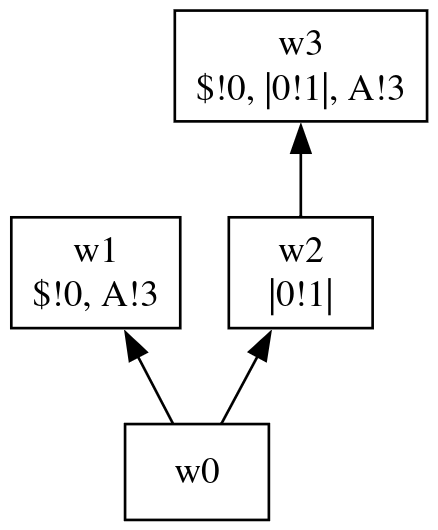
\includegraphics[width=0.3\textwidth]{invalid-peirce.png}
  \caption{Контрмодель Kripke для схемы Пирса}
  \label{fig:peirce-cm}
\end{figure}

\subsection{Невалидная формула: исключённое третье}

\textbf{Вход} (\verb|examples/formulas/invalid-excluded-middle.txt|):
\verb+A \/ -A+

\textbf{Полученные клозы} (после клозификации):
\begin{itemize}
  \item \textbf{R} (flat): \verb+(A => $)+
  \item \textbf{X} (impl): \verb+((A => _|_) => $)+
\end{itemize}

\textbf{Результат:} контрмодель Kripke (рис.~\ref{fig:em-cm}).

\begin{figure}[htbp]
  \centering
  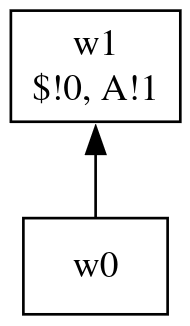
\includegraphics[width=0.17\textwidth]{invalid-excluded-middle.png}
  \caption{Контрмодель Kripke для формулы $A \lor \lnot A$}
  \label{fig:em-cm}
\end{figure}

\subsection{Невалидная формула: закон де Моргана для дизъюнкции}

\textbf{Вход} (\verb|examples/formulas/invalid-de-morgan-or.txt|):
\verb+-(A /\ B) => (-A \/ -B)+

\textbf{Полученные клозы} (после клозификации):
\begin{itemize}
  \item \textbf{R} (flat): \verb+(_|_ => 1)+, \verb+((0 /\ A /\ B) => _|_)+
  \item \textbf{X} (impl): \verb+((B => _|_) => 1)+, \verb+((A => _|_) => 1)+,
        \verb+((0 => 1) => $)+
\end{itemize}

\textbf{Результат:} контрмодель Kripke (рис.~\ref{fig:demorgan-cm}); формула невалидна
(не выводится \texttt{Valid}).

\begin{figure}[htbp]
  \centering
  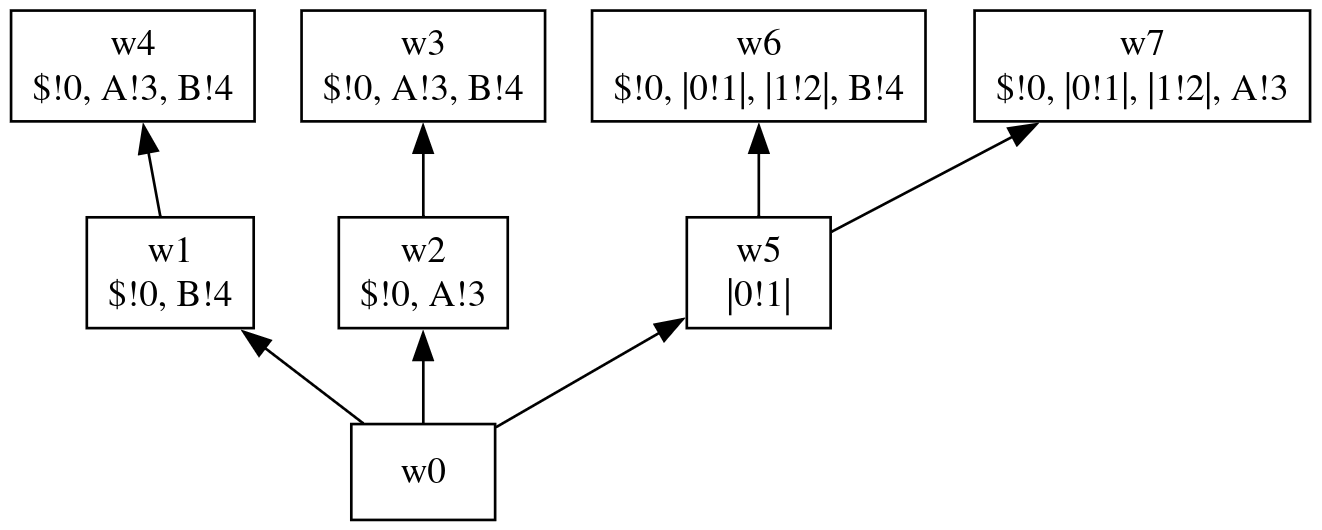
\includegraphics[width=0.72\textwidth]{invalid-de-morgan.png}
  \caption{Контрмодель Kripke для \texttt{-(A /\ B) => (-A \/ -B)}}
  \label{fig:demorgan-cm}
\end{figure}

\subsection{Сложный валидный пример}

\textbf{Вход} (\verb|examples/formulas/complex-and-impl-chain.txt|):
\begin{lstlisting}[style=formula,caption={Сложная валидная формула с цепочкой импликаций},label={lst:ex-complex}]
(((a /\ (b /\ c) /\ d) => c) => a) => a
\end{lstlisting}

\textbf{Результат:} \texttt{Valid}, длинная цепочка клозификации (AsFlat,
RightCs, AsImpl, Aliasing, RightImpl, \ldots) и соответствующий граф
\texttt{digraph Proof}.

\textbf{Результирующий терм:}
\begin{lstlisting}[caption={Редуцированный $\lambda$-терм для сложной формулы},label={lst:ex-complex-term}]
($62(\$25.($25(\$40.(P(4)$40)))))
\end{lstlisting}

\subsection{Сложный валидный пример: вложенная схема Пирса}

\textbf{Вход} (\verb|examples/formulas/complex-peirce-nested.txt|):
\begin{lstlisting}[style=formula,caption={Вложенная схема Пирса},label={lst:ex-peirce-nested}]
((((a => b) => a) => a) => b) => b
\end{lstlisting}

\textbf{Результат:} \texttt{Valid}. Клозификация включает несколько шагов
\texttt{Aliasing}, \texttt{RightImpl}, \texttt{AsFlat}, \texttt{AsImpl} и три
применения \texttt{ImplImpliesFlat}; доказательство в CArrow использует CPL0 и CPL1.

\textbf{Результирующий терм:}
\begin{lstlisting}[caption={Редуцированный $\lambda$-терм для вложенной схемы Пирса},label={lst:ex-peirce-nested-term}]
($58(\$28.($28(\$37.($37(\$43.($28K($43))))))))
\end{lstlisting}

\subsection{Сложный валидный пример: syj201}

\textbf{Вход} (\verb|examples/formulas/syj201.txt|). Формула состоит из трёх
посылок (взаимная импликация пары переменных $\Rightarrow$ конъюнкция $a \land b \land c$)
и заключения $a \land b \land c$:
\begin{lstlisting}[style=formula,breaklines=true,caption={Формула syj201 (разбита по строкам)},label={lst:ex-syj201}]
(
  ((a => b) /\ (b => a) => (a /\ b /\ c))
  /\
  ((b => c) /\ (c => b) => (a /\ b /\ c))
  /\
  ((c => a) /\ (a => c) => (a /\ b /\ c))
) => (a /\ b /\ c)
\end{lstlisting}

\textbf{Полученные клозы} (после клозификации):
\hssnippet{syj201-clauses.txt}{Итоговые клозы для syj201}

\textbf{Результат:} \texttt{Valid}. Доказательство в CArrow использует множество
шагов CPL1.

\textbf{Результирующий терм:}
\begin{lstlisting}[breaklines=true,caption={Редуцированный $\lambda$-терм для syj201},label={lst:ex-syj201-term}]
($624(\$195.<(P(3)((P(1)$195)(\$378.(P(2)((P(3)$195)K($378)))))),(P(2)((P(3)$195)K((P(3)((P(3)$195)(\$506.(P(3)((P(2)$195)(\$553.(P(2)((P(3)$195)K($506)))))))))))),(P(1)((P(3)$195)K((P(3)((P(3)$195)(\$506.(P(3)((P(2)$195)(\$553.(P(2)((P(3)$195)K($506))))))))))))>))
\end{lstlisting}

\end{document}
